\documentclass[12pt,a4paper]{article}
\usepackage[utf8]{inputenc}
\usepackage[indonesian]{babel}
\usepackage[margin=2.5cm]{geometry}
\usepackage{graphicx}
\usepackage{booktabs}
\usepackage{longtable}
\usepackage{listings}
\usepackage{xcolor}
\usepackage{hyperref}

\definecolor{codegreen}{rgb}{0,0.6,0}
\definecolor{codegray}{rgb}{0.5,0.5,0.5}
\definecolor{codepurple}{rgb}{0.58,0,0.82}
\definecolor{backcolour}{rgb}{0.95,0.95,0.92}

\lstdefinestyle{sql}{
  language=SQL,
  backgroundcolor=\color{backcolour},
  commentstyle=\color{codegreen},
  keywordstyle=\color{blue}\bfseries,
  numberstyle=\tiny\color{codegray},
  stringstyle=\color{codepurple},
  basicstyle=\ttfamily\footnotesize,
  breaklines=true,
  frame=single,
  numbers=left,
  numbersep=8pt,
  columns=flexible,
  showstringspaces=false
}

\title{\textbf{Laporan Praktikum}\\
       Basis Data — Week 5\\
       \large Fungsi dan Basis Data (PostgreSQL)}
\author{Romi\\
        Program Studi Sistem Informasi\\
        Semester 3 — Pemrograman Basis Data}
\date{\today}

\begin{document}
\maketitle
\thispagestyle{empty}

\begin{abstract}
Praktikum ini membahas pembuatan dan pemanfaatan \emph{fungsi} (stored function)
pada basis data, meliputi fungsi skalar murni, fungsi yang membaca tabel,
penerapan dalam laporan, pengujian, penelusuran galat, pengukuran kinerja, dan
pengelolaan fungsi. Seluruh praktikum dijalankan pada \textbf{PostgreSQL 18};
soal aslinya ditulis untuk MySQL sehingga dilakukan penyesuaian sintaks
(tabel perbandingan pada Bagian~\ref{sec:adaptasi}).
\end{abstract}

\tableofcontents
\newpage

% ============================ PERSIAPAN ============================
\section{Persiapan}

\subsection{Pemeriksaan Lingkungan}
\begin{lstlisting}[style=sql]
SELECT VERSION();
SELECT CURRENT_USER, CURRENT_DATABASE;
\end{lstlisting}

PostgreSQL tidak memiliki perintah \texttt{SHOW GRANTS FOR CURRENT\_USER()} maupun
variabel \texttt{log\_bin\_trust\_function\_creators}; keduanya khas MySQL. Galat
nomor 1418 (khusus MySQL) tidak muncul di PostgreSQL.

\subsection{Basis Data Kerja (P1--P4)}
Dibuat database \texttt{db\_fungsi\_hr} dengan empat tabel operasional
(\texttt{pegawai}, \texttt{departemen}, \texttt{penempatan}, \texttt{gaji}) dan satu
tabel pengujian \texttt{uji\_fungsi}. Data diisi dari dataset asli
\texttt{employees} melalui \emph{foreign table}.

\begin{center}
\begin{tabular}{lrrrr}
\toprule
departemen & pegawai & penempatan & gaji & uji\_fungsi\\
\midrule
9 & 5000 & 5524 & 47603 & 16\\
\bottomrule
\end{tabular}
\end{center}

\begin{center}
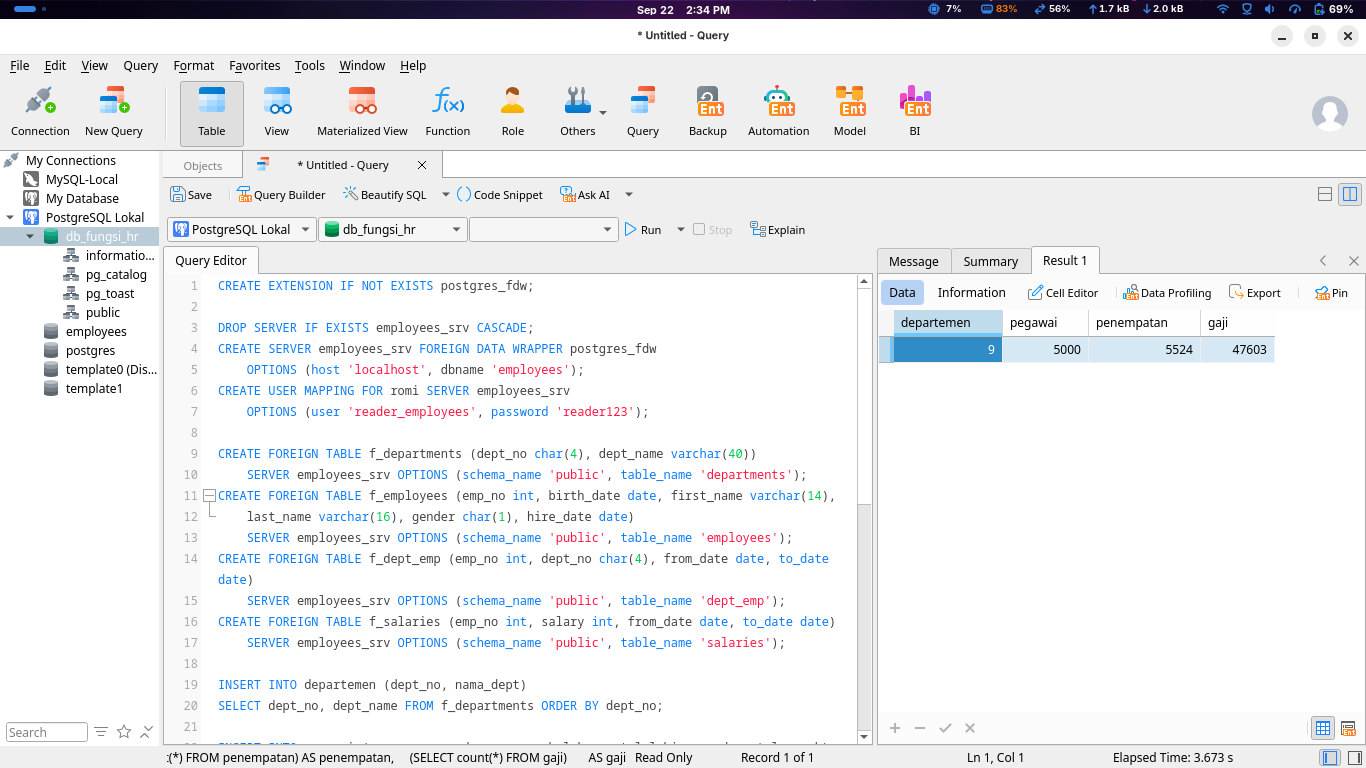
\includegraphics[width=0.9\textwidth]{screenshot/ss_03_jumlah_baris.png}
\captionof{figure}{Jumlah baris keempat tabel operasional (P3).}
\end{center}

% ============================ BAGIAN B ============================
\section{Fungsi Skalar Murni (Bagian B)}

Enam fungsi dibuat: \texttt{fn\_usia}, \texttt{fn\_masa\_kerja},
\texttt{fn\_masa\_kerja\_teks}, \texttt{fn\_rapikan\_nama},
\texttt{fn\_format\_rupiah}, dan \texttt{fn\_kategori\_gaji} (dengan helper
\texttt{fn\_group\_thousands}). Contoh fungsi \texttt{fn\_usia}:

\begin{lstlisting}[style=sql]
CREATE OR REPLACE FUNCTION fn_usia(p_tgl_lahir DATE)
RETURNS INT LANGUAGE plpgsql IMMUTABLE AS $$
DECLARE v_usia INT;
BEGIN
  IF p_tgl_lahir IS NULL THEN RETURN NULL; END IF;
  IF p_tgl_lahir > CURRENT_DATE THEN
     RAISE EXCEPTION 'tanggal lahir tidak valid: %', p_tgl_lahir;
  END IF;
  v_usia := EXTRACT(YEAR FROM AGE(CURRENT_DATE, p_tgl_lahir));
  RETURN v_usia;
END; $$;
\end{lstlisting}

Uji (B7) dilakukan dengan nilai normal, \texttt{NULL}, dan nilai tidak wajar
(tanggal masa depan, nama kosong, gaji negatif). Fungsi mengembalikan
\texttt{NULL} untuk \texttt{NULL} input dan menolak input tak valid dengan
\texttt{RAISE EXCEPTION}.

\begin{center}
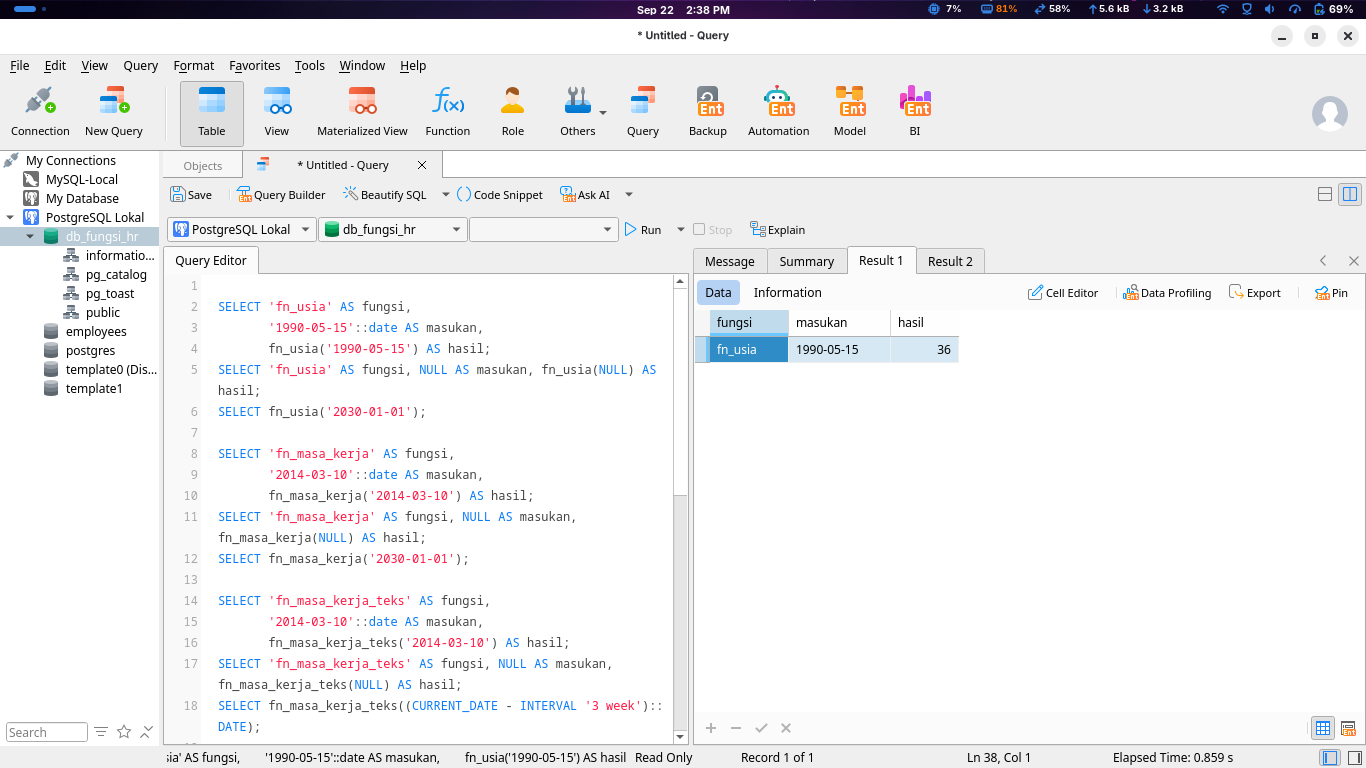
\includegraphics[width=0.9\textwidth]{screenshot/ss_06_uji_B.png}
\captionof{figure}{Hasil pengujian fungsi Bagian B.}
\end{center}

\subsection{Pertanyaan Analisis B}
\texttt{fn\_usia} bergantung pada \texttt{CURRENT\_DATE}, sehingga hasilnya berubah
seiring waktu. Bila dipaksa \texttt{IMMUTABLE} (padanan \texttt{DETERMINISTIC}),
mesin basis data boleh meng-cache hasilnya: pada \textbf{replikasi}, node yang
memakai hasil cache akan menampilkan usia yang usang/tidak konsisten; dan
\textbf{hasil query yang disimpan sementara} (view materialized, common
subexpression) akan membeku dan tidak terupdate saat tanggal berganti. Maka fungsi
ini tidak boleh dideklarasikan \texttt{IMMUTABLE}.

% ============================ BAGIAN C ============================
\section{Fungsi yang Membaca Tabel (Bagian C)}

Lima fungsi \texttt{STABLE}: \texttt{fn\_gaji\_berjalan}, \texttt{fn\_nama\_dept},
\texttt{fn\_gaji\_rata\_dept}, \texttt{fn\_peringkat\_gaji} (memanggil dua fungsi
lain), dan \texttt{fn\_total\_kenaikan}. Diuji dengan tiga jenis \texttt{emp\_no}:

\begin{center}
\begin{tabular}{llrrrl}
\toprule
Jenis & emp\_no & gaji\_berjalan & nama\_dept & peringkat & total\_kenaikan\\
\midrule
A (lengkap)              & 10001 & 88958 & Development       & Di Atas Rata-rata & 28841\\
B (tanpa gaji berjalan)  & 10008 & NULL  & Tidak Ditempatkan & Tidak Ada Gaji    & 5997\\
C (tidak ada)            & 99999 & NULL  & Tidak Ditempatkan & Tidak Ada Gaji    & 0\\
\bottomrule
\end{tabular}
\end{center}

\begin{center}
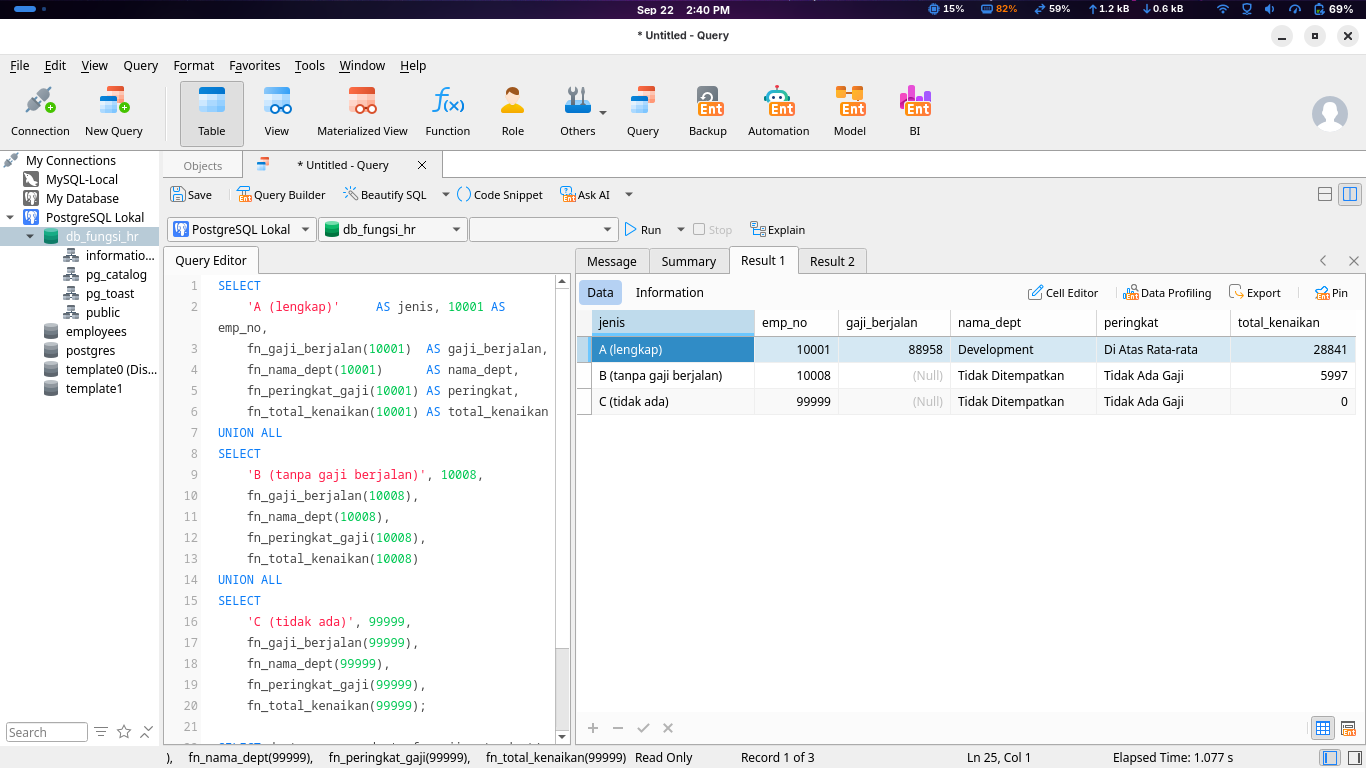
\includegraphics[width=0.9\textwidth]{screenshot/ss_08_uji_C.png}
\captionof{figure}{Pengujian fungsi Bagian C dengan tiga jenis masukan.}
\end{center}

\subsection{Pertanyaan Analisis C}
Penyusunan berlapis memberi (1) \emph{reuse \& konsistensi} — logika ditulis sekali,
dipakai di mana saja; (2) \emph{keterbacaan \& pemeliharaan} — query laporan pendek
dan aturan cukup diubah di satu tempat. Risikonya: \emph{kinerja \& ketergantungan
berantai} — tiap lapisan menambah panggilan (memperlambat), dan perubahan/
penghapusan fungsi dasar berdampak kaskade ke semua pemanggil.

% ============================ BAGIAN D ============================
\section{Penerapan dalam Skenario Nyata (Bagian D)}

\subsection*{D1 — Profil Pegawai}
Laporan 50 baris; seluruh kolom turunan berasal dari pemanggilan fungsi.

\begin{center}
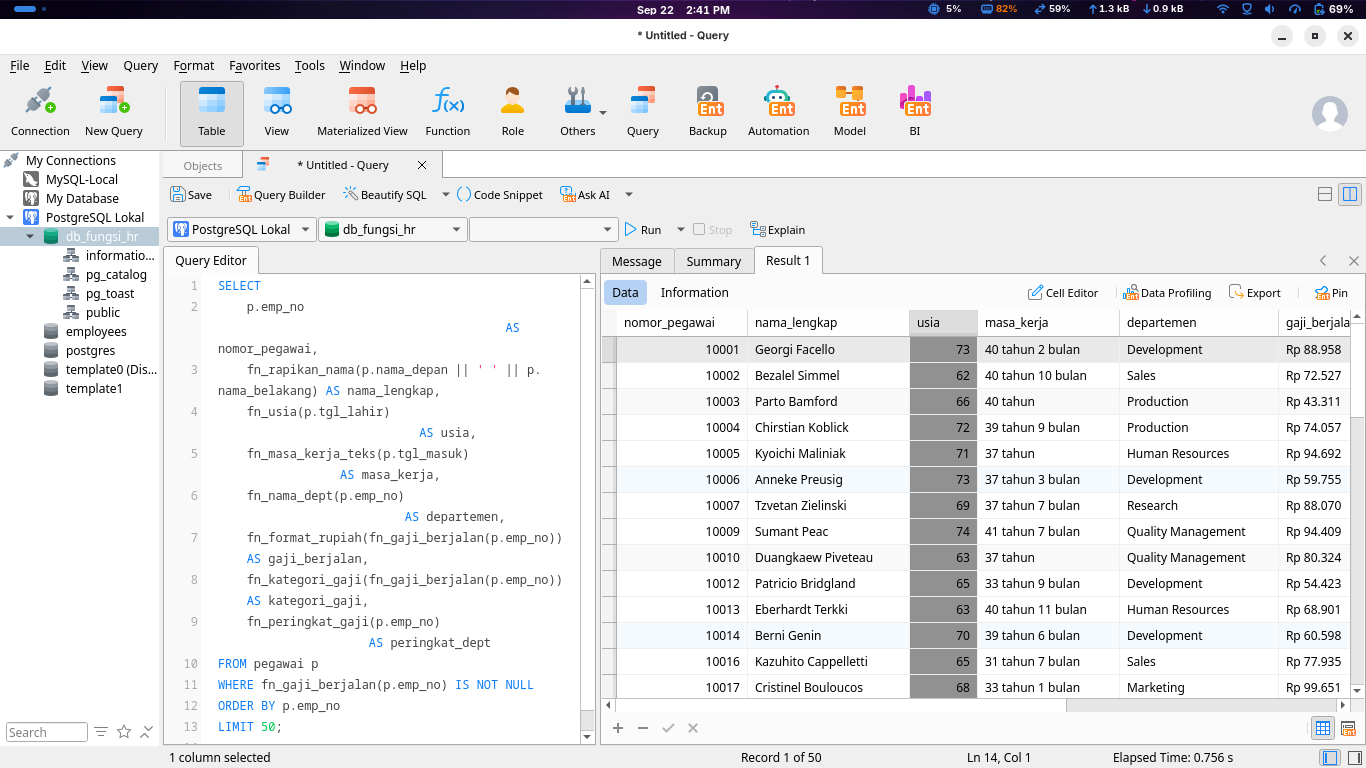
\includegraphics[width=0.95\textwidth]{screenshot/ss_09_D1_profil.png}
\captionof{figure}{Laporan profil pegawai (D1).}
\end{center}

\subsection*{D2 — Proyeksi Pensiun}
Query memakai \texttt{fn\_usia} di \texttt{WHERE} dan \texttt{ORDER BY}. Pada dataset
ini seluruh pegawai berusia 61--74 tahun (sudah melewati 60), sehingga hasil
\textbf{0 baris} — temuan ini dilaporkan apa adanya beserta bukti sebaran usia.

\begin{center}
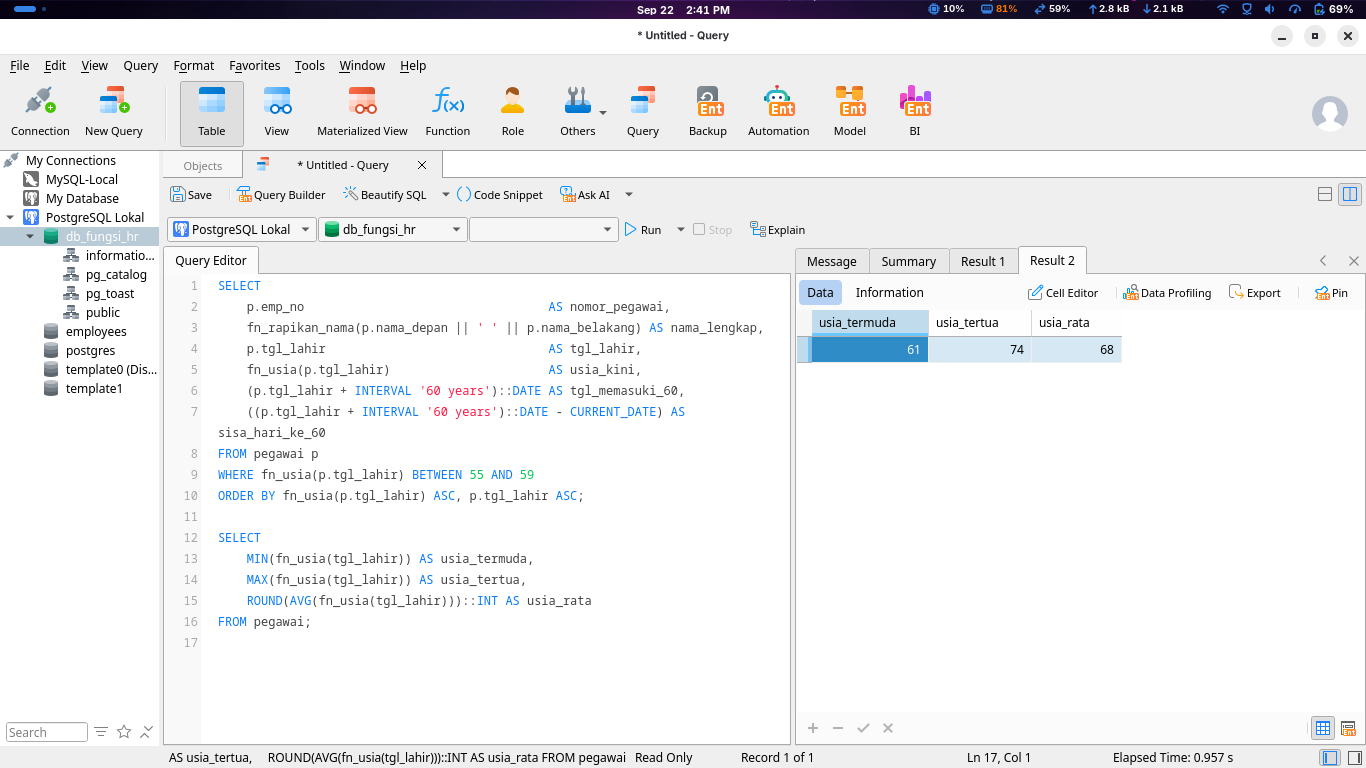
\includegraphics[width=0.9\textwidth]{screenshot/ss_10_D2_pensiun.png}
\captionof{figure}{Proyeksi pensiun (D2) — 0 baris karena pegawai sudah $>$60 tahun.}
\end{center}

\subsection*{D3 — Rekap per Departemen}
\begin{center}
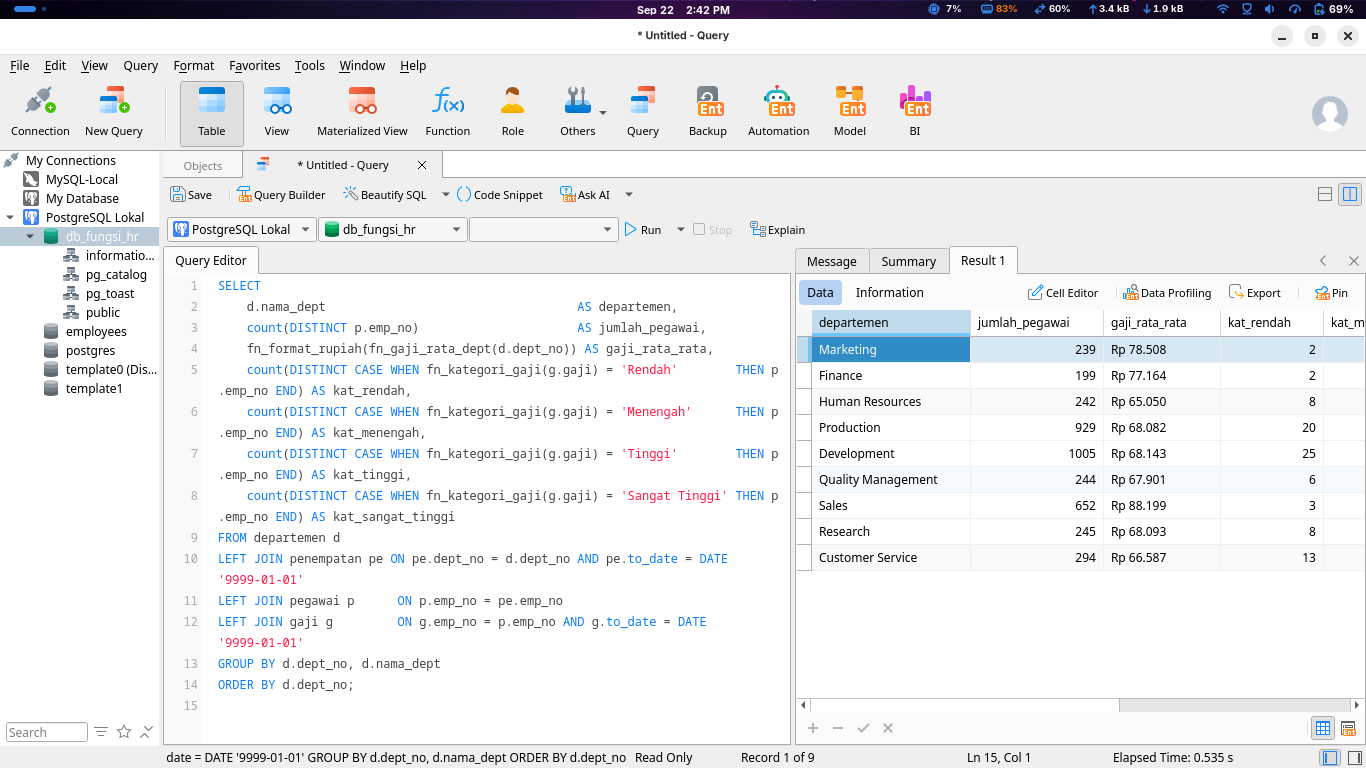
\includegraphics[width=0.95\textwidth]{screenshot/ss_11_D3_rekap.png}
\captionof{figure}{Rekapitulasi per departemen (D3).}
\end{center}

\subsection*{D4 \& D5 — Validasi Gaji dan Trigger}
\texttt{fn\_validasi\_gaji} mengembalikan \texttt{'VALID'} atau pesan penolakan.
Trigger \texttt{BEFORE UPDATE} \texttt{trg\_cek\_gaji} menolak perubahan bila hasil
validasi bukan \texttt{'VALID'} (memakai \texttt{RAISE EXCEPTION} = padanan
\texttt{SIGNAL SQLSTATE '45000'}).

\begin{center}
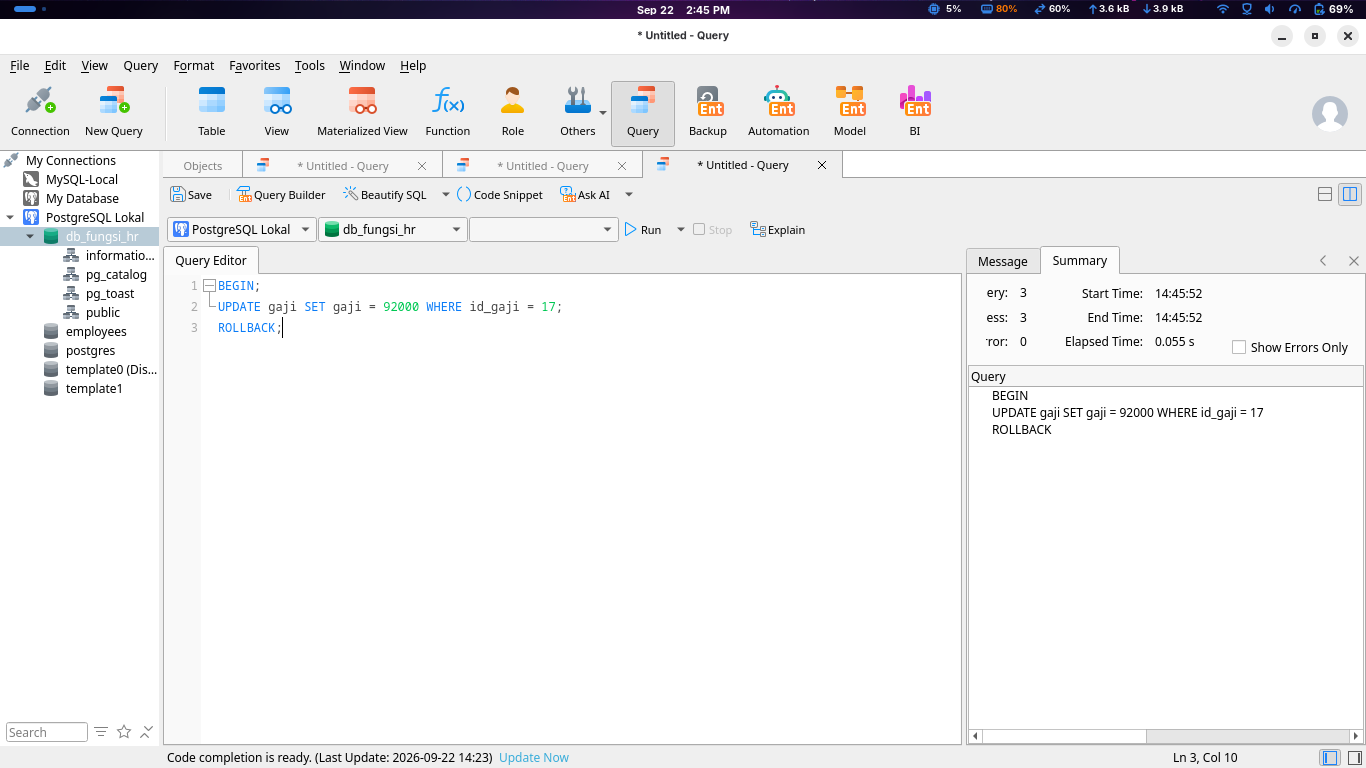
\includegraphics[width=0.9\textwidth]{screenshot/ss_14_D5_trigger_uji.png}
\captionof{figure}{Trigger menolak UPDATE yang tidak valid (ERROR) dan mengizinkan yang valid.}
\end{center}

\subsection*{D6 — View}
\texttt{v\_profil\_pegawai} membungkus query D1 sehingga cukup
\texttt{SELECT * FROM v\_profil\_pegawai}.

\begin{center}
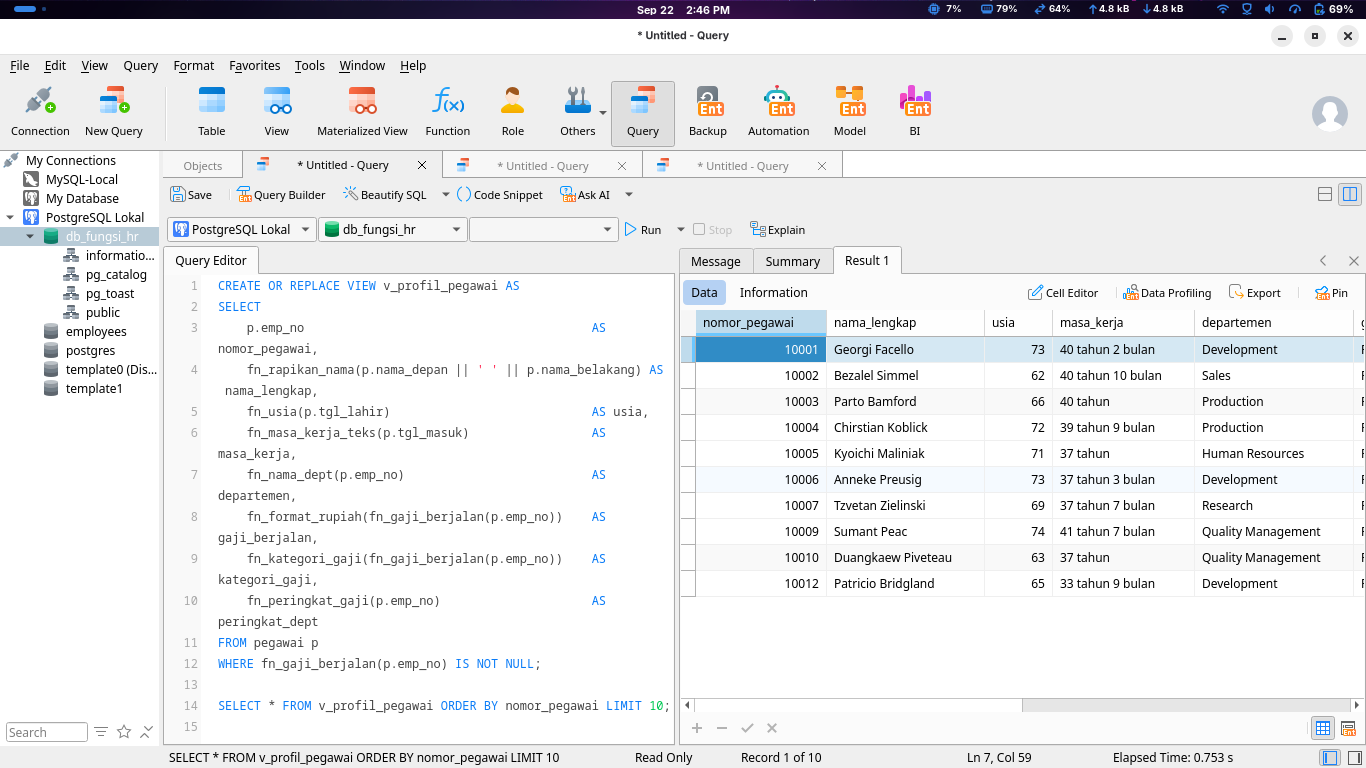
\includegraphics[width=0.9\textwidth]{screenshot/ss_15_D6_view.png}
\captionof{figure}{Pemanggilan view v\_profil\_pegawai (D6).}
\end{center}

\subsection{Pertanyaan Analisis D}
\begin{itemize}
  \item \textbf{Fungsi} — terbaik untuk logika kompleks/bersyarat dengan parameter,
        mis. \texttt{fn\_validasi\_gaji} yang dipakai trigger \& query.
  \item \textbf{View} — terbaik untuk presentasi berulang yang selalu ``live'',
        mis. \texttt{v\_profil\_pegawai}.
  \item \textbf{Generated column} — terbaik untuk nilai turunan stabil yang sering
        difilter/disortir karena tersimpan fisik dan bisa diindeks.
\end{itemize}

% ============================ BAGIAN E ============================
\section{Pengujian, Penelusuran, dan Pengelolaan (Bagian E)}

\subsection*{E1 — Inventaris Fungsi}
\begin{center}
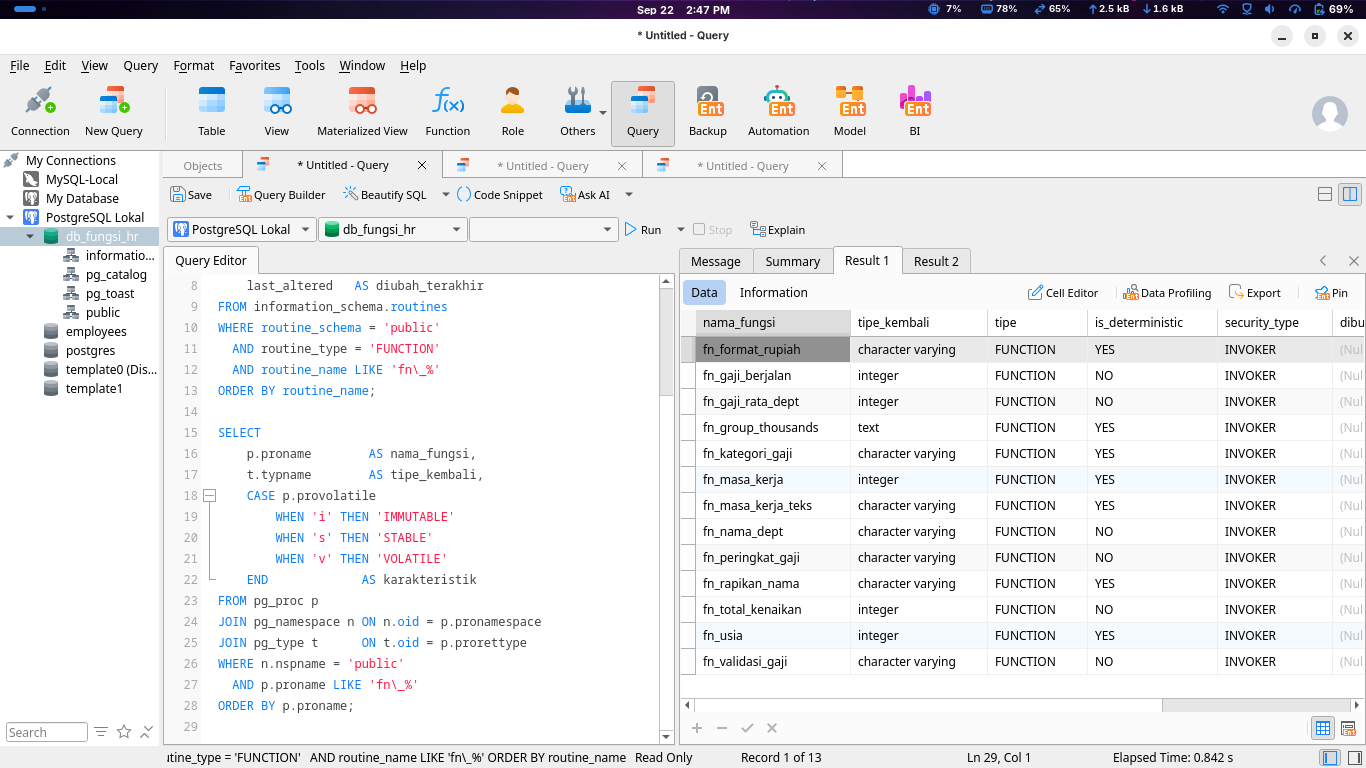
\includegraphics[width=0.9\textwidth]{screenshot/ss_16_E1_inventaris.png}
\captionof{figure}{Inventaris fungsi via information\_schema.ROUTINES.}
\end{center}

\subsection*{E2 — Pengujian Terpusat}
16 kasus uji dicatat di \texttt{uji\_fungsi}; \textbf{semuanya LULUS} (16 lulus, 0 gagal).

\begin{center}
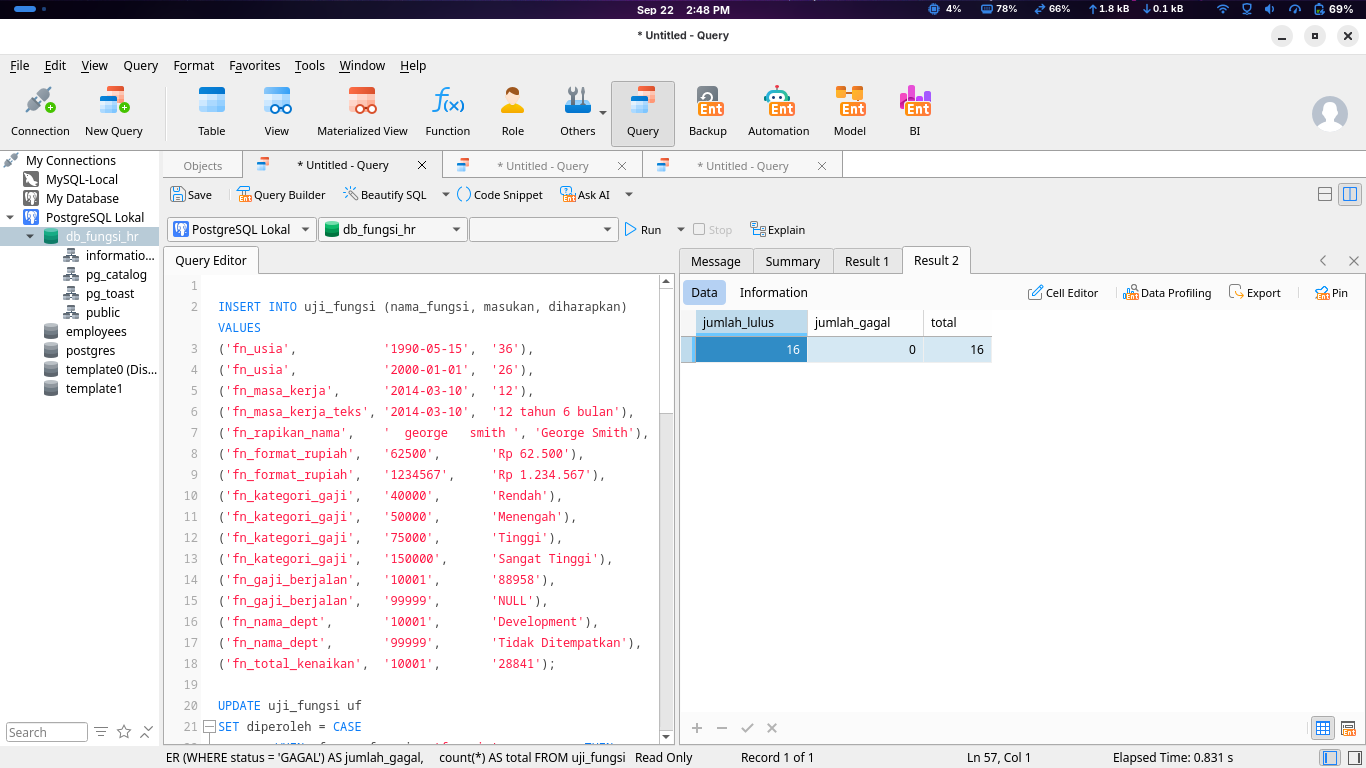
\includegraphics[width=0.9\textwidth]{screenshot/ss_17_E2_uji.png}
\captionof{figure}{Rekapitulasi hasil pengujian (E2).}
\end{center}

\subsection*{E3 — Penelusuran Galat}
Skrip \texttt{fn\_bonus} yang diberikan mengandung enam kesalahan:
(1) \texttt{v\_bonus} tidak dideklarasikan; (2) tidak ada \texttt{RETURN};
(3) \texttt{SELECT ... INTO} tanpa \texttt{LIMIT} (error bila $>$1 baris);
(4) tidak menangani \texttt{NULL} pada \texttt{v\_gaji}; (5) pengali desimal pada
variabel \texttt{INT} memotong presisi; (6) penggunaan \texttt{DELIMITER} yang tidak
dikenali PostgreSQL. Versi perbaikan disajikan pada file \texttt{42\_E3\_debug.sql}.

\subsection*{E4 \& E5 — Pengukuran Kinerja}
\begin{center}
\begin{tabular}{lrr}
\toprule
Ukuran & Kolom/JOIN langsung & Ber-fungsi\\
\midrule
E4 (5000 baris) & 9.8 ms  & 30.6 ms\\
E5 (rekap dept) & 35 ms   & 79 ms\\
\bottomrule
\end{tabular}
\end{center}

\begin{center}
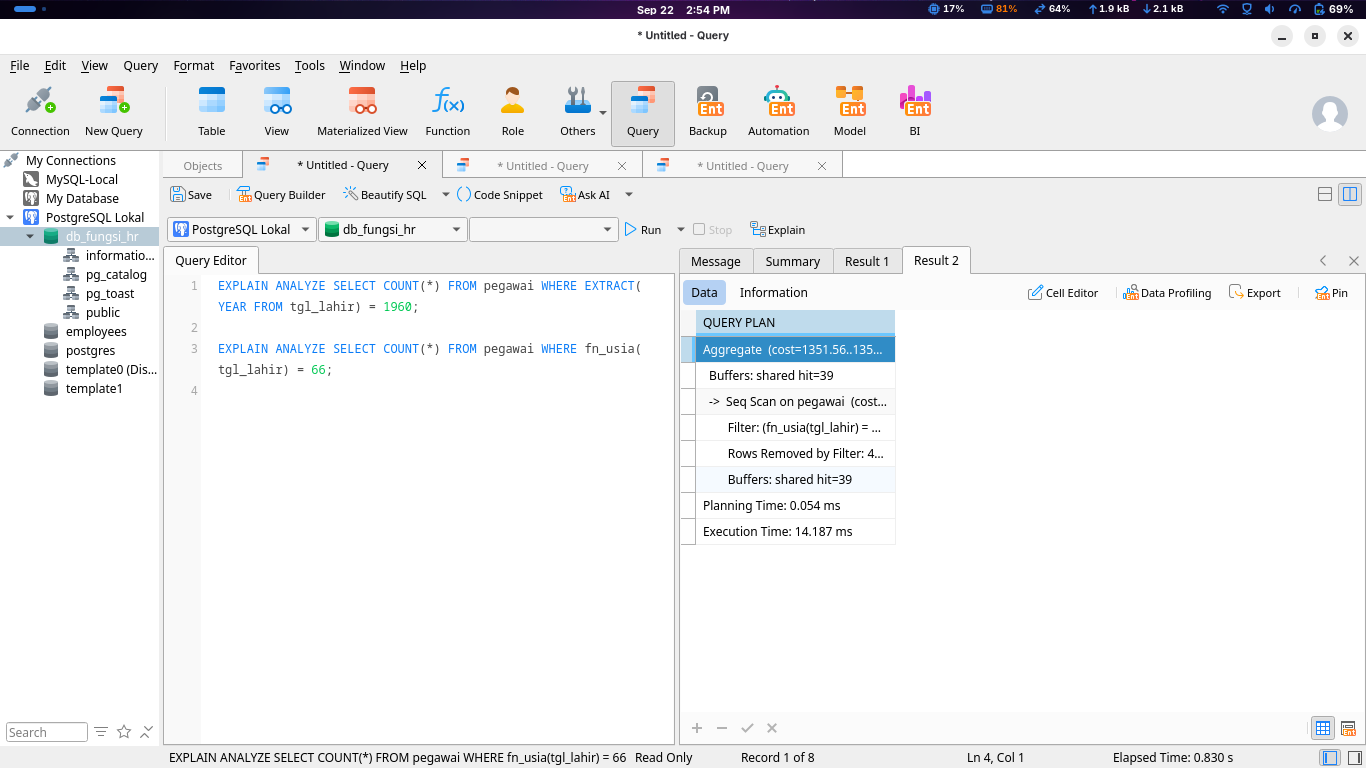
\includegraphics[width=0.9\textwidth]{screenshot/ss_19_E4_benchmark.png}
\captionof{figure}{Benchmark E4 — \texttt{EXPLAIN} menunjukkan Seq Scan pada keduanya.}
\end{center}

Predikat yang membungkus kolom dengan fungsi membuat \textbf{indeks pada kolom
mentah tidak terpakai} (Seq Scan). Untuk tetap memakai indeks diperlukan
\emph{expression index} pada ekspresi tersebut.

\subsection*{E7 — Faktorial}
PostgreSQL tidak mendukung rekursi fungsi; faktorial diimplementasikan dengan loop
iteratif \texttt{FOR}.

\begin{center}
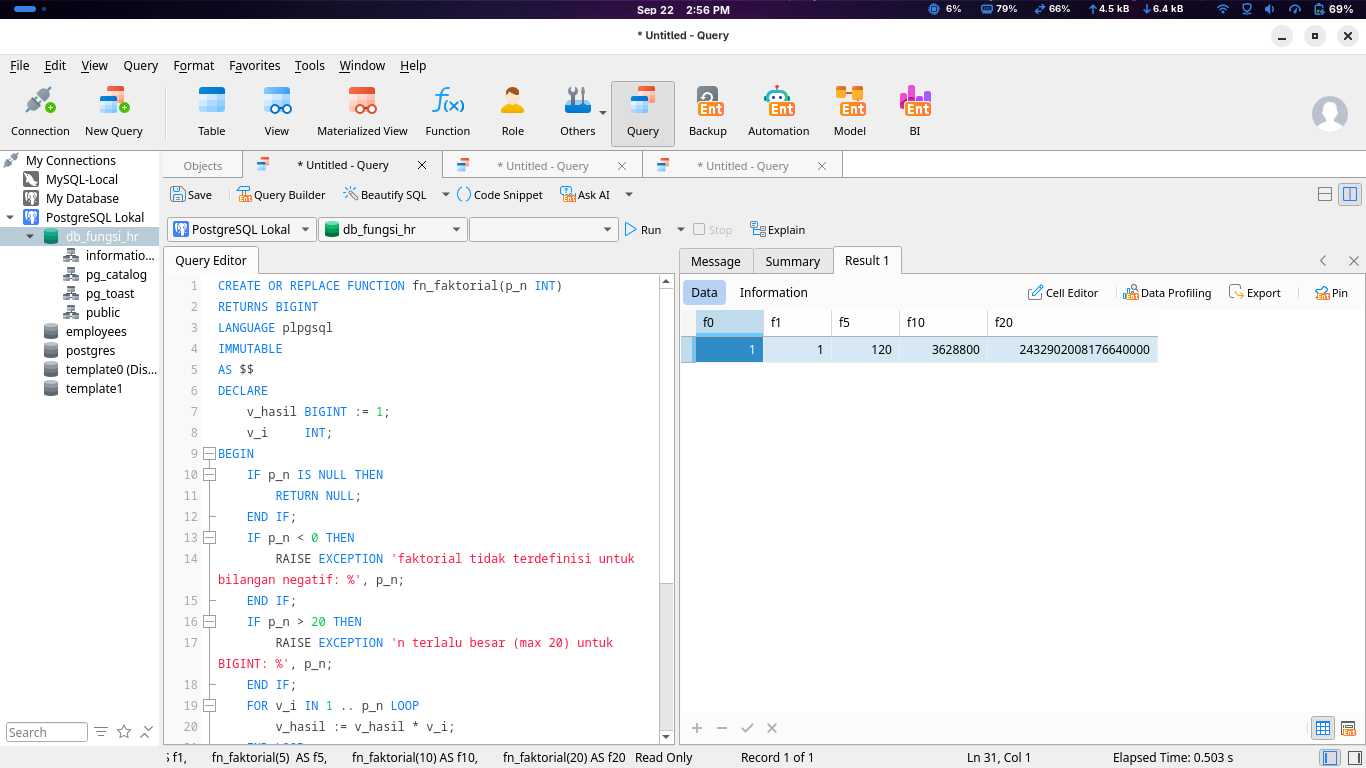
\includegraphics[width=0.8\textwidth]{screenshot/ss_21_E7_faktorial.png}
\captionof{figure}{Hasil fn\_faktorial (E7).}
\end{center}

\subsection{Pertanyaan Analisis E}
Dua teknik penelusuran logika fungsi:
(1) \texttt{RAISE NOTICE/INFO/DEBUG} — ringan, namun keluaran masuk ke log dan
bising bila berlebihan; (2) menyimpan jejak ke tabel audit — lebih terstruktur,
namun menambah I/O dan menyisihkan efek (tidak cocok untuk fungsi
\texttt{IMMUTABLE/STABLE}).

% ============================ TUGAS TAMBAHAN ============================
\section{Tugas Tambahan (G1--G3)}

\subsection*{G1 — Terbilang}
\texttt{fn\_terbilang} mengubah bilangan menjadi kata Indonesia s.d. jutaan.
Contoh: \texttt{62500} $\rightarrow$ ``enam puluh dua ribu lima ratus''.

\begin{center}
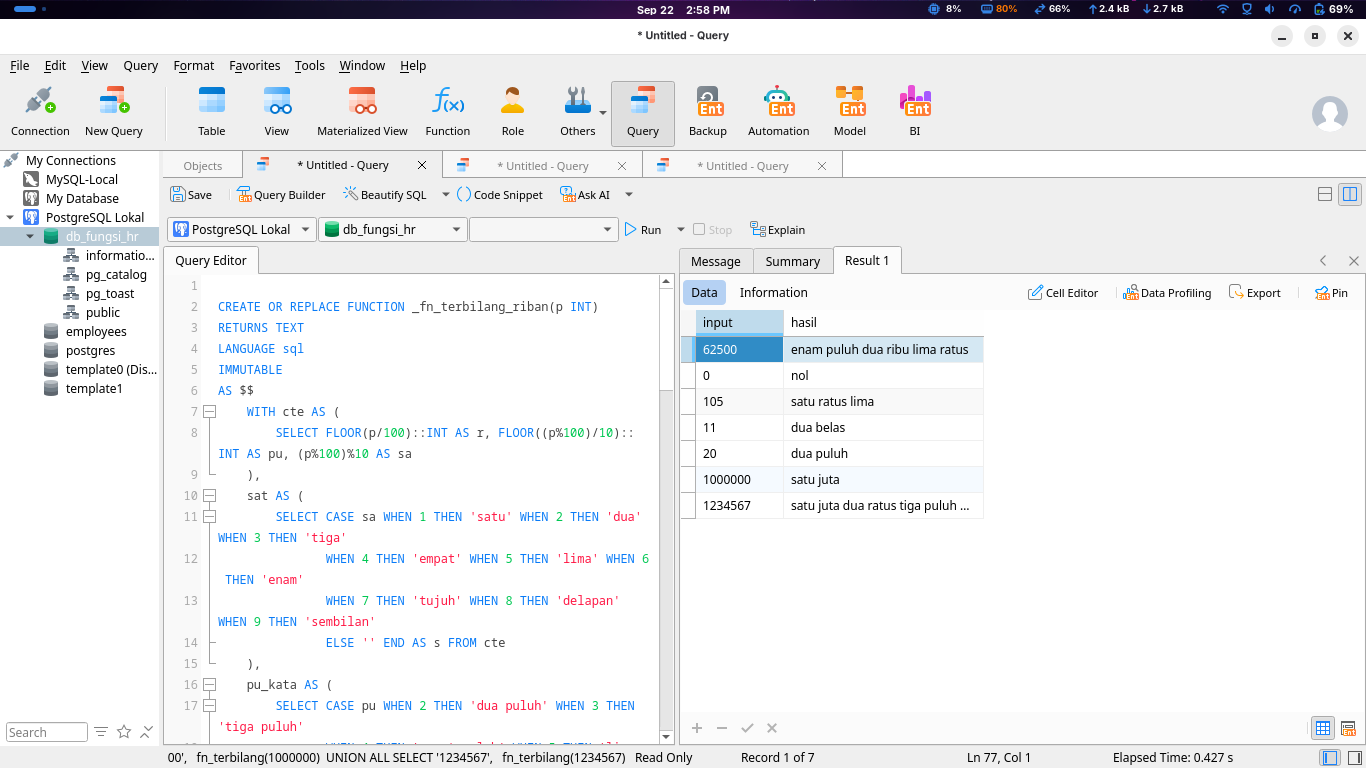
\includegraphics[width=0.9\textwidth]{screenshot/ss_22_G1_terbilang.png}
\captionof{figure}{Hasil fn\_terbilang (G1).}
\end{center}

\subsection*{G2 — Hari Kerja}
\texttt{fn\_hari\_kerja} menghitung hari kerja (Sen--Jum) dengan rumus matematis
(minggu penuh $\times$ 5 + sisa), tanpa perulangan baris-per-baris.

\begin{center}
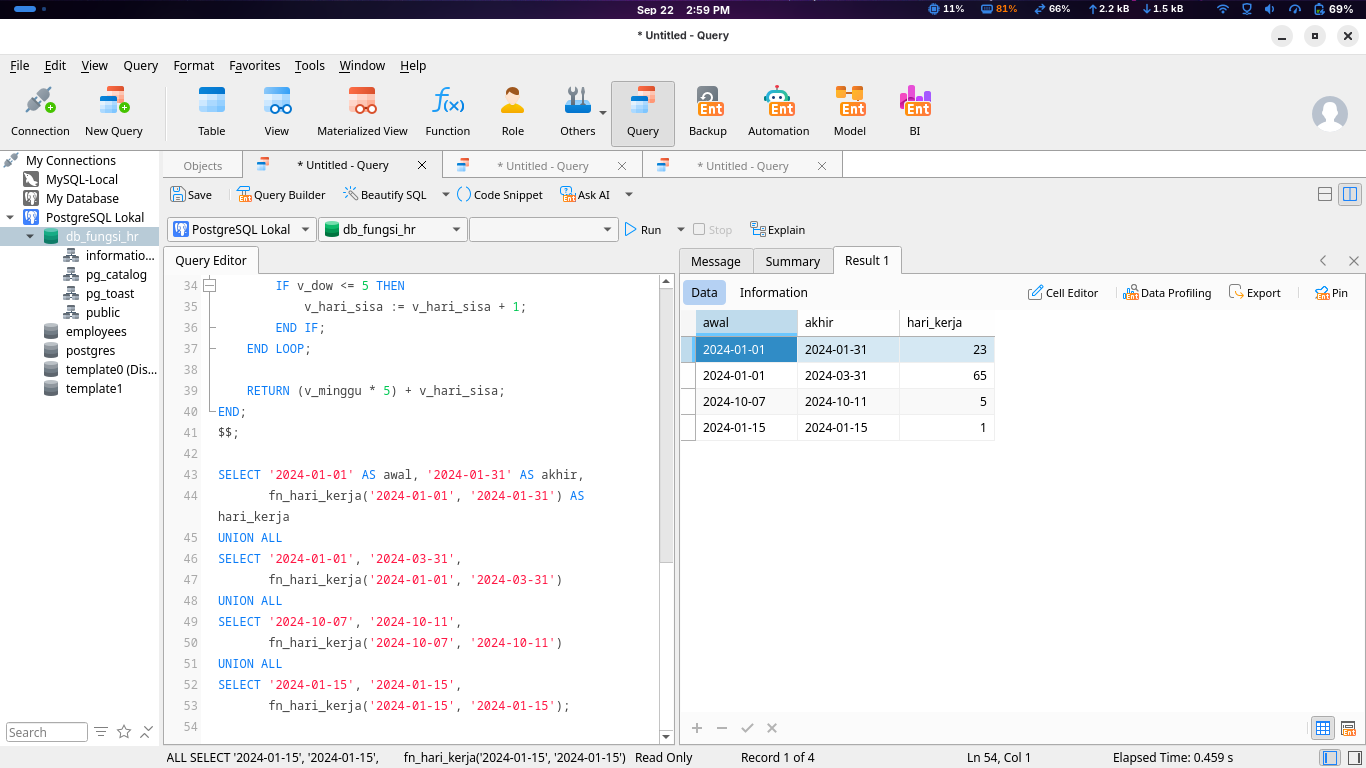
\includegraphics[width=0.9\textwidth]{screenshot/ss_23_G2_hari_kerja.png}
\captionof{figure}{Hasil fn\_hari\_kerja (G2).}
\end{center}

\subsection*{G3 — Caching}
Mekanisme caching \texttt{fn\_gaji\_rata\_dept} menggunakan tabel
\texttt{cache\_gaji\_rata\_dept} dengan masa kedaluwarsa 1 jam. Kinerja naik dari
\textbf{79 ms menjadi 2 ms} (hasil identik). Risikonya: bila data gaji berubah
dalam jendela 1 jam, cache menyajikan nilai yang \emph{usang} sampai kedaluwarsa.

\begin{center}
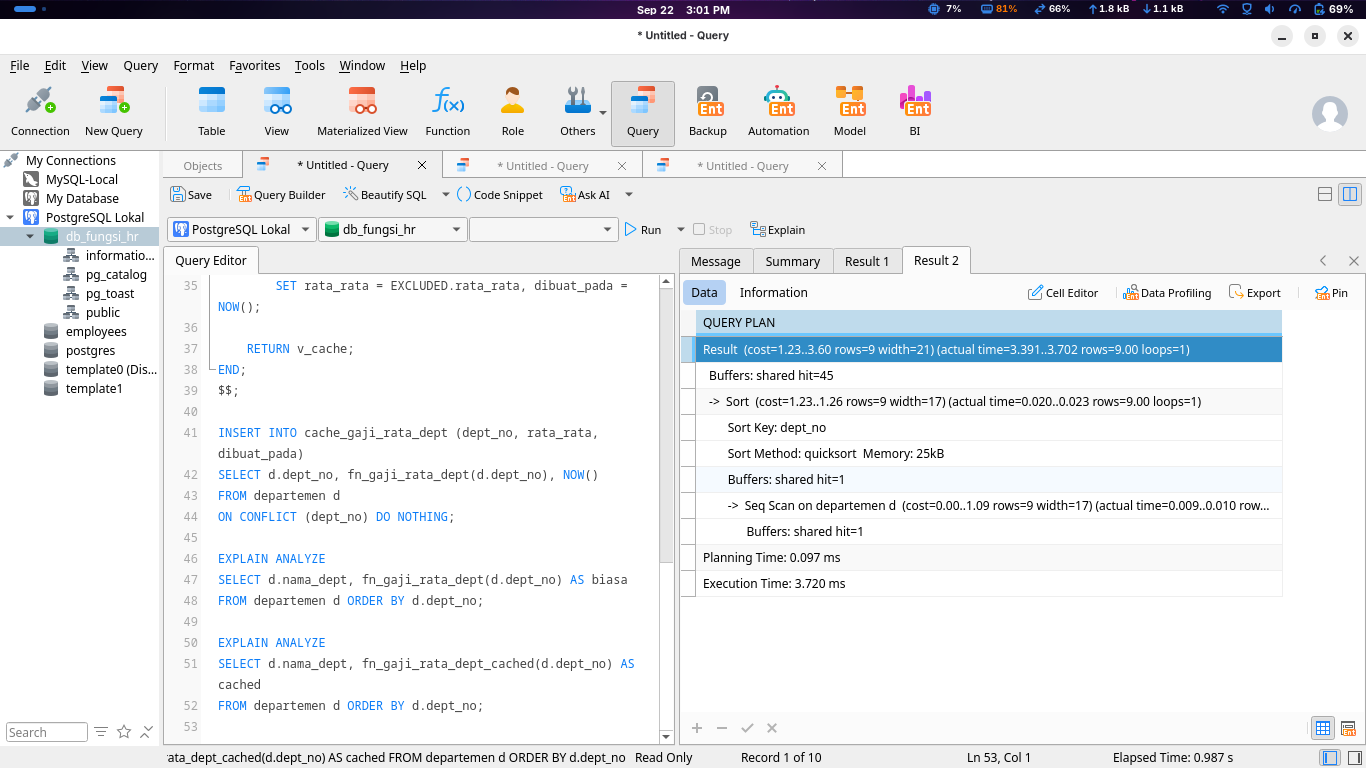
\includegraphics[width=0.9\textwidth]{screenshot/ss_24_G3_caching.png}
\captionof{figure}{Benchmark caching (G3): 79 ms $\rightarrow$ 2 ms.}
\end{center}

% ============================ ADAPTASI ============================
\section{Penyesuaian MySQL $\rightarrow$ PostgreSQL}\label{sec:adaptasi}

\begin{center}
\begin{tabular}{ll}
\toprule
MySQL (di soal) & PostgreSQL (dipakai)\\
\midrule
\texttt{AUTO\_INCREMENT} & \texttt{GENERATED ALWAYS AS IDENTITY}\\
\texttt{DELIMITER \$\$ ...} & body langsung \texttt{AS \$\$ ... \$\$}\\
\texttt{SHOW FUNCTION STATUS} & \texttt{information\_schema.ROUTINES}/\texttt{pg\_proc}\\
\texttt{SIGNAL SQLSTATE '45000'} & \texttt{RAISE EXCEPTION}\\
\texttt{DETERMINISTIC}/\texttt{READS SQL DATA} & \texttt{IMMUTABLE}/\texttt{STABLE}/\texttt{VOLATILE}\\
Error 1418 + \texttt{log\_bin\_trust\_function\_creators} & tidak ada padanan (khas MySQL)\\
\texttt{YEAR(tgl)}, \texttt{CURDATE()} & \texttt{EXTRACT(YEAR FROM ...)}, \texttt{CURRENT\_DATE}\\
\texttt{USE db;} & pilih database (tanpa \texttt{USE})\\
\bottomrule
\end{tabular}
\end{center}

% ============================ SIMPULAN ============================
\section{Simpulan}
Fungsi basis data sangat berguna untuk menyusun logika bisnis yang berulang menjadi
pendek, seragam, dan mudah dibaca. Namun fungsi yang membungkus kolom pada data
besar menurunkan kinerja karena indeks tidak terpakai; untuk kasus agregat berulang
yang mahal, caching terbukti memberi percepatan signifikan (79 ms $\rightarrow$
2 ms). Tiga pedoman: pakai fungsi untuk logika kompleks, hindari fungsi di predikat
kolom besar, dan gunakan caching/generated column untuk agregat berulang.

\end{document}
